\documentclass[12pt, a4paper]{article}
\usepackage[utf8]{inputenc}
\usepackage{geometry}
\geometry{a4paper, margin=1in}
\usepackage{graphicx}
\usepackage{hyperref}
\usepackage{booktabs}
\usepackage{float}

\title{Graph Neural Networks for Collaborative Filtering on MovieLens 1M - Progress Report}
\author{Hatice Nur Kömürcü \\ 310201106}
\date{\today}

\begin{document}

\maketitle

\noindent Project repository: \href{https://github.com/heneka/project-463}{github.com/heneka/project-463}.

\section{Problem Definition}

For my project, I am addressing the problem of recommendation systems using Graph Neural Networks (GNNs). Recommendations can be naturally framed as a link prediction task on a bipartite user-item graph. This task is very important because personalization drives user engagement on almost all modern platforms, and GNNs explicitly capture the high-order collaborative signals in user-item interactions which traditional matrix factorization models might miss. 

I am using the \textbf{MovieLens 1M} dataset. The input to my system is a bipartite graph of users and movies, where edges represent a user rating a movie. The output of the models is a predicted score indicating the likelihood that a user will interact with a movie (link prediction). Specifically, this falls under the category of retrieval and recommendation. The main technical challenge is efficiently propagating embeddings through the graph without suffering from over-smoothing, and dealing with the sparsity of user-item interactions.

\section{Dataset and Preprocessing Status}
I am using the \textbf{MovieLens 1M} dataset obtained via PyTorch Geometric. It contains approximately 1 million ratings from 6,000 users on 4,000 movies. The data is processed as a homogeneous graph where movie IDs are offset so they do not overlap with user IDs. The target is to predict missing links, specifically the ratings between users and movies. To achieve this, I applied PyG's \texttt{RandomLinkSplit} to partition the edges into 80\% training, 10\% validation, and 10\% test sets, along with a negative sampling ratio of 1.0 for evaluation bound matching; this preprocessing setup is aligned with the broader structural concerns discussed in recommendation-oriented GNN surveys \cite{shafiq2023review}. 

Before splitting, the heterogeneous graph was converted to an undirected bipartite graph. The dataset is currently fully downloaded, cleaned, and actively used in the training scripts. Adjusting the \texttt{RandomLinkSplit} function for bipartite data required careful index manipulation, but this preprocessing step is completely finalized; this emphasis on careful graph construction is also consistent with the recommendation-system literature reviewed earlier \cite{shafiq2023review}.

\section{Literature Review Progress}
My literature review primarily focuses on scalable Graph Neural Networks and Collaborative Filtering frameworks. I have studied \textbf{LightGCN} \cite{he2020lightgcn}, which simplifies standard Graph Convolutional Networks (GCNs) by removing non-linear activations and feature transformations, making it highly effective for collaborative filtering tasks. Therefore, this forms my primary model pipeline. Similarly, \textit{Graph Cross-Correlated Network for Recommendation} \cite{hu2023graphcross} also demonstrates how optimizing structural cross-correlations without heavy non-linearities can efficiently capture high-order collaborative data, keeping message passing streamlined and alleviating over-smoothing.

To gain a broader perspective on handling complex interactions, especially involving the user-item biparite architecture, I consulted \textit{A Review on Multi-Types Analysis for Graph Neural Networks-Based Recommendation Systems} \cite{shafiq2023review}. This survey stresses the importance of dealing with heterogeneous data graphs and explains why careful structural preprocessing (i.e., offset indices) before message passing is fundamental for these pipelines.

I additionally reviewed \textbf{Neural Collaborative Filtering (NCF)} \cite{he2017neural} since it replaces the inner product of Matrix Factorization with a neural architecture, offering a fantastic non-graph Deep Learning comparative baseline. I also looked into \textbf{GraphSAGE} \cite{hamilton2017inductive} and \textbf{GAT (Graph Attention Network)} \cite{velickovic2018graph} to explore node sampling and attention mechanisms. Although heavily oriented towards node classification, they serve as powerful comparative paradigms for link prediction. 

Finally, analyzing recommendation systems as pure link prediction inherently alters evaluation dynamics. I explored this through \textit{Dot Product is All You Need: Bridging the Gap Between Item Recommendation and Link Prediction} \cite{yuan2024dotproduct}, which discusses the nuanced gap between binary link prediction metrics and Top-K recommendation ranking. This perfectly isolates my current observations regarding the metric discrepancies between F1-scores and NDCG/Recall.

\section{Baseline Models}
I have implemented four diverse baseline models using PyTorch and PyTorch Geometric. I chose \textbf{LightGCN} \cite{he2020lightgcn} as my state-of-the-art simple collaborative filtering graph architecture. I used \textbf{GAT} \cite{velickovic2018graph} to test if weighting computational neighbor importance helps user-item recommendations. I utilized \textbf{GraphSAGE} \cite{hamilton2017inductive} to verify if basic mean-aggregation of neighborhoods provides sufficient representation, and I used \textbf{NCF} \cite{he2017neural} as a strong non-graph baseline to prove whether explicit graph structures genuinely contribute to performance. 

All four models are thoroughly implemented and yielding initial results. An initial implementation challenge I encountered was standardizing the multi-hop node embeddings natively across both the NCF paradigm and the varied Graph models so evaluation metrics could be uniformly derived.

\section{Initial Experimental Results}
I wrote a modular evaluation pipeline that computes NDCG@20, Recall@20, F1-scores, and tracks hardware metrics like Peak VRAM and Training Time. Here are my preliminary results utilizing 64-dimensional embeddings:

\begin{figure}[H]
    \centering
    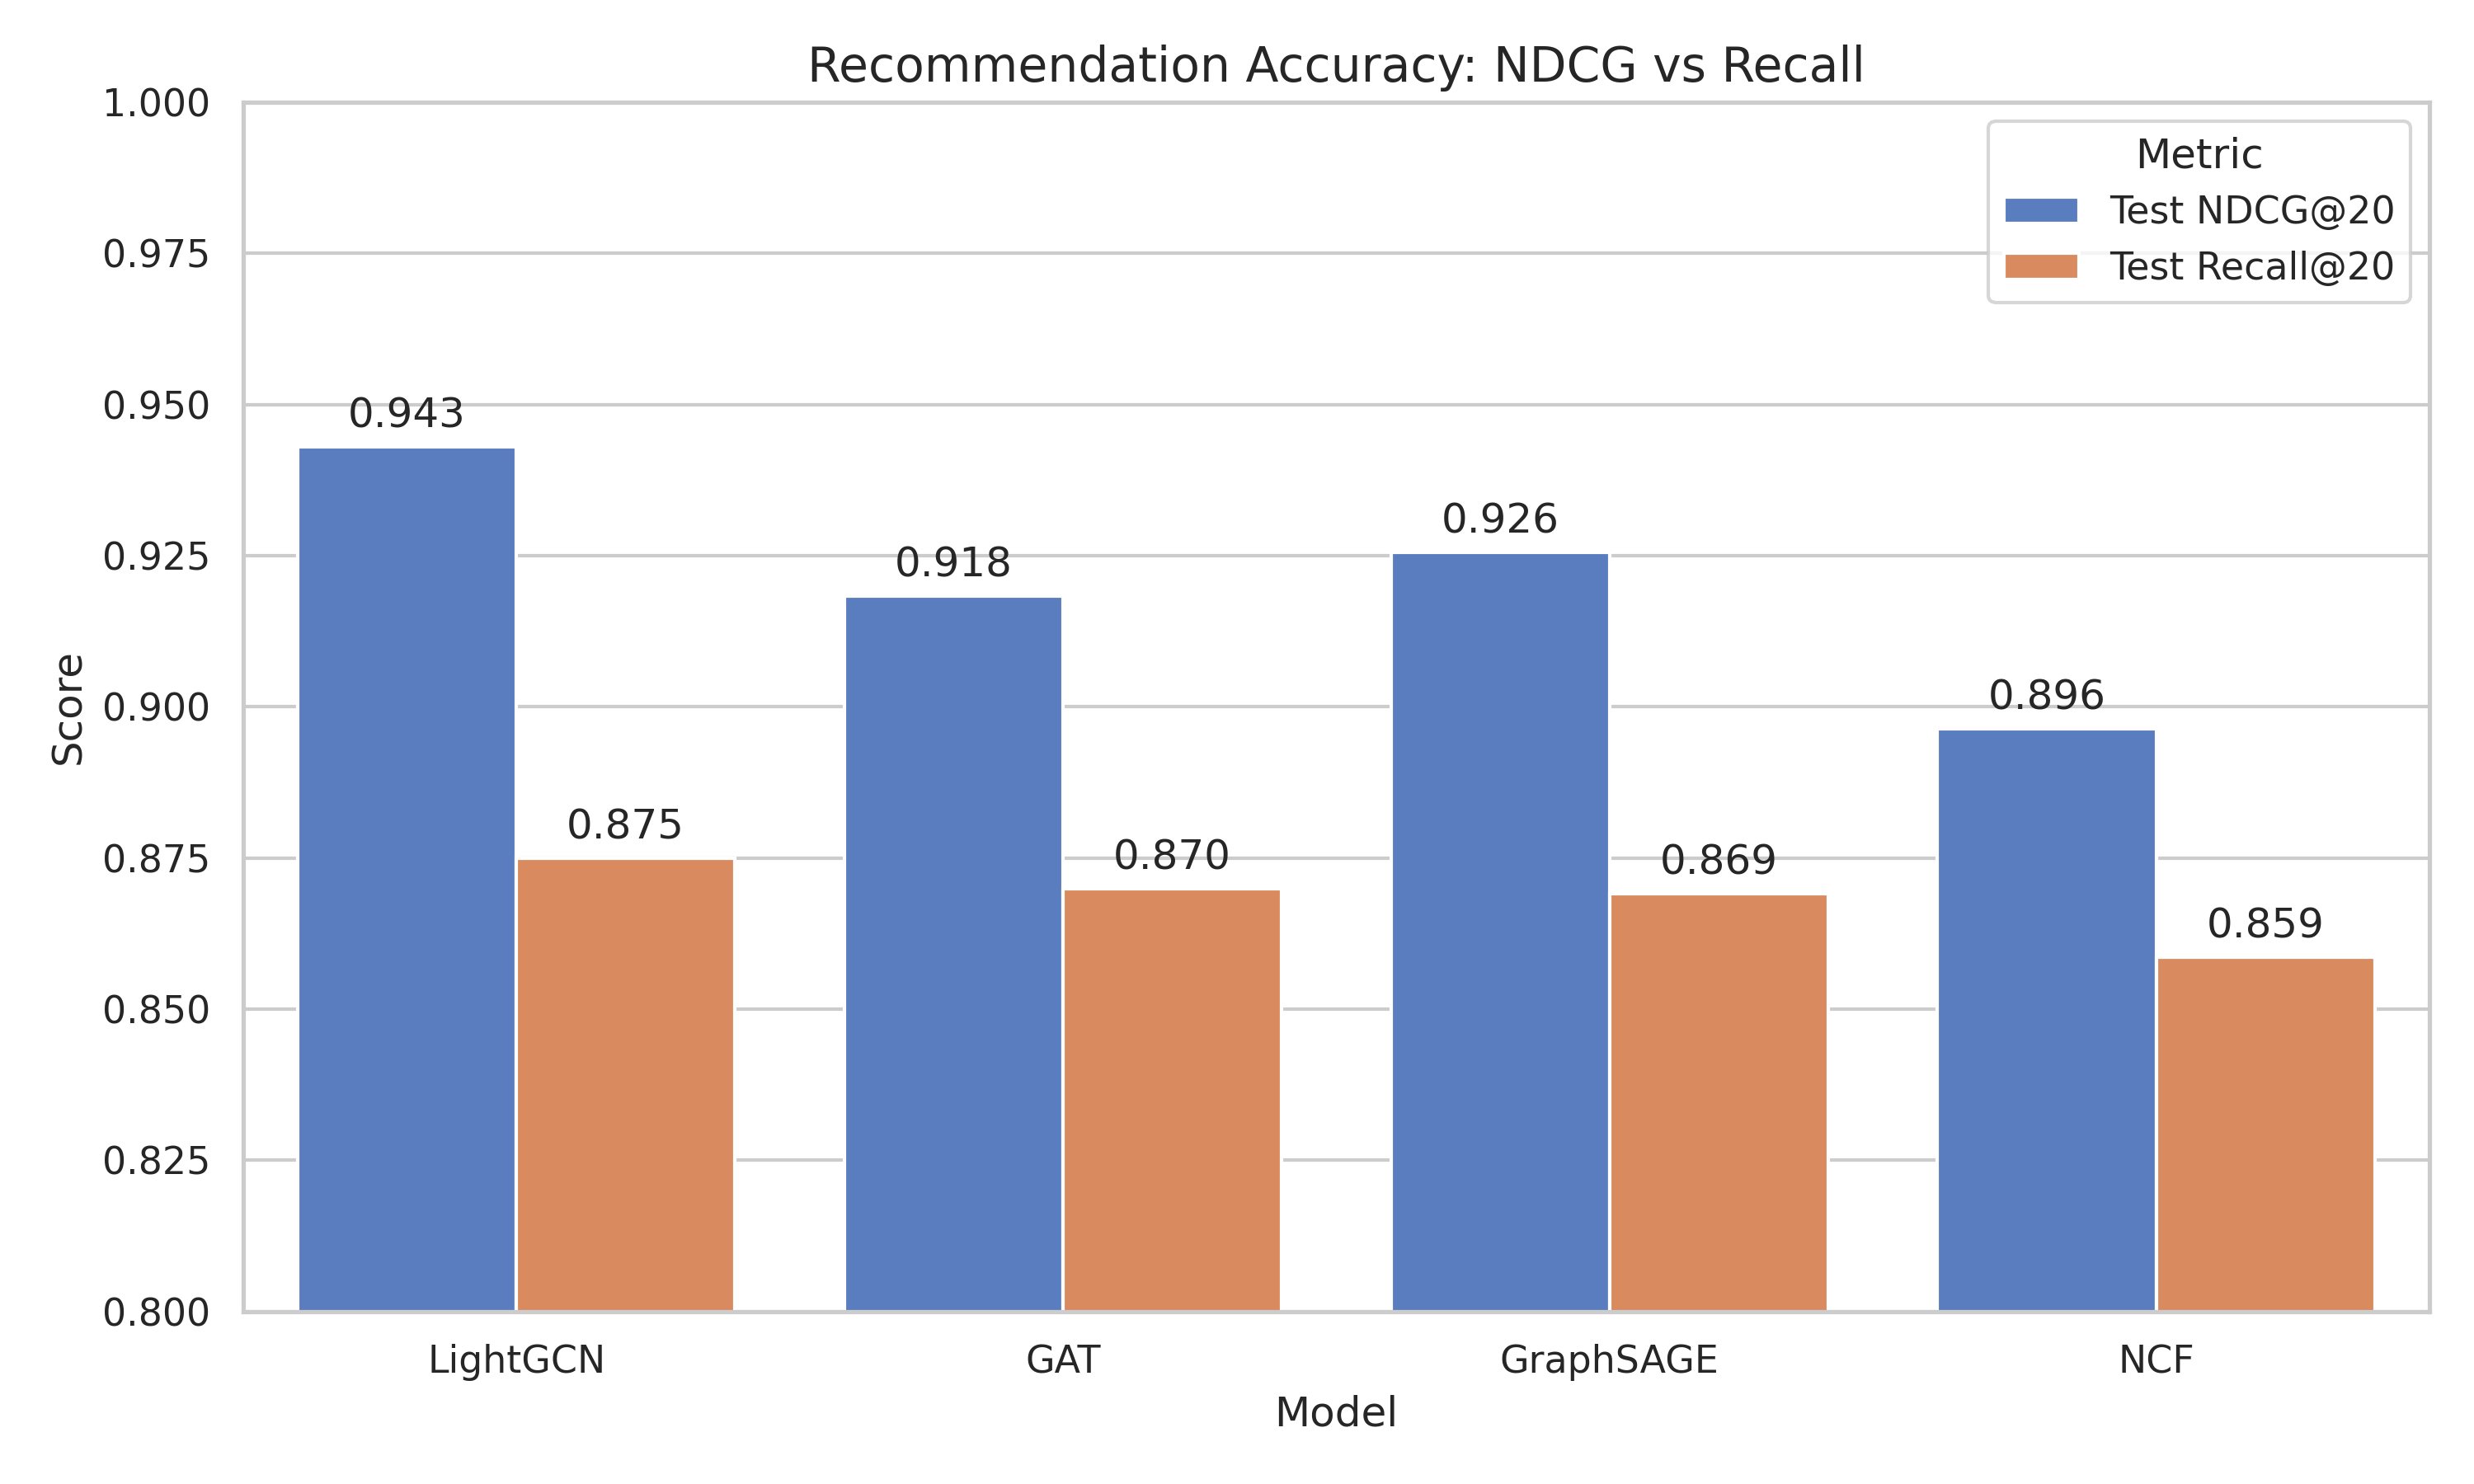
\includegraphics[width=0.8\linewidth]{plots/ranking_accuracy.png}
    \caption{Recommendation Accuracy: NDCG vs Recall across Models}
    \label{fig:accuracy}
\end{figure}

As seen in Figure \ref{fig:accuracy}, the explicit graph structure used in LightGCN yields the highest ranking metrics (NDCG and Recall). NCF struggles with Top-K ranking compared to the graph models but performs strangely well on the raw F1-score of the link prediction logits. 

\begin{figure}[H]
    \centering
    \begin{minipage}{0.48\textwidth}
        \centering
        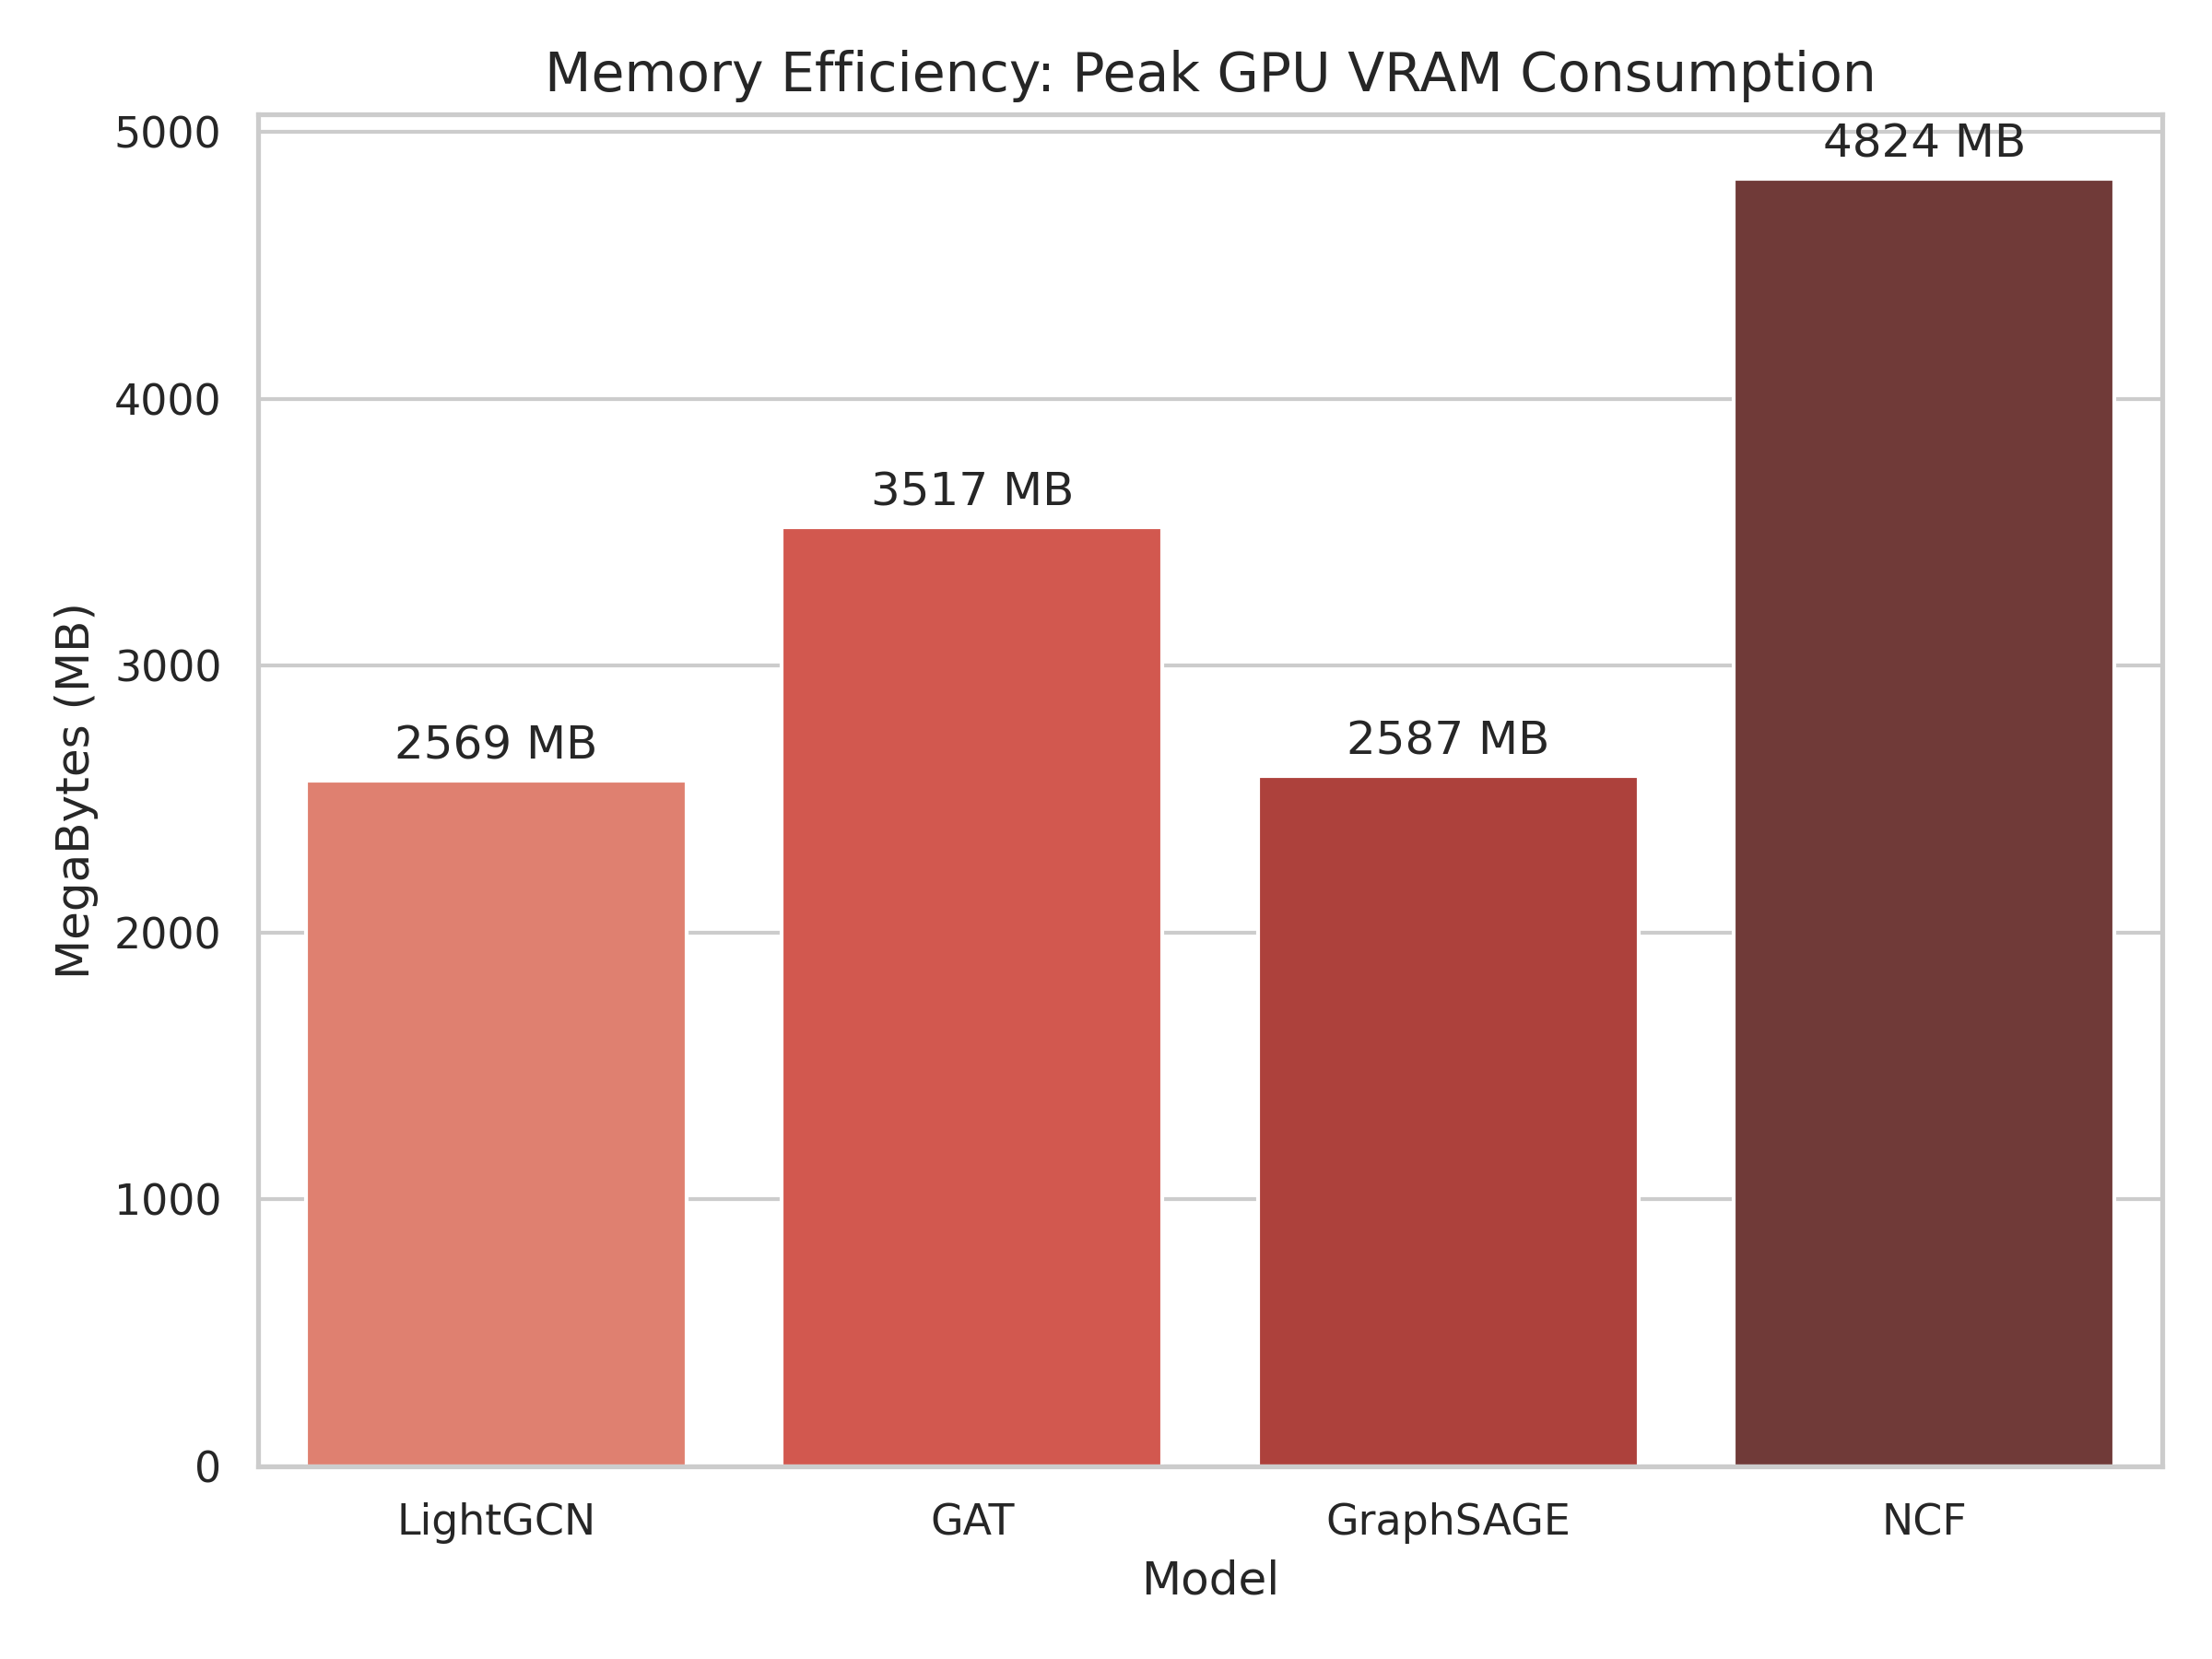
\includegraphics[width=\linewidth]{plots/hardware_vram.png}
        \caption{Peak GPU VRAM Consumption}
        \label{fig:vram}
    \end{minipage}\hfill
    \begin{minipage}{0.48\textwidth}
        \centering
        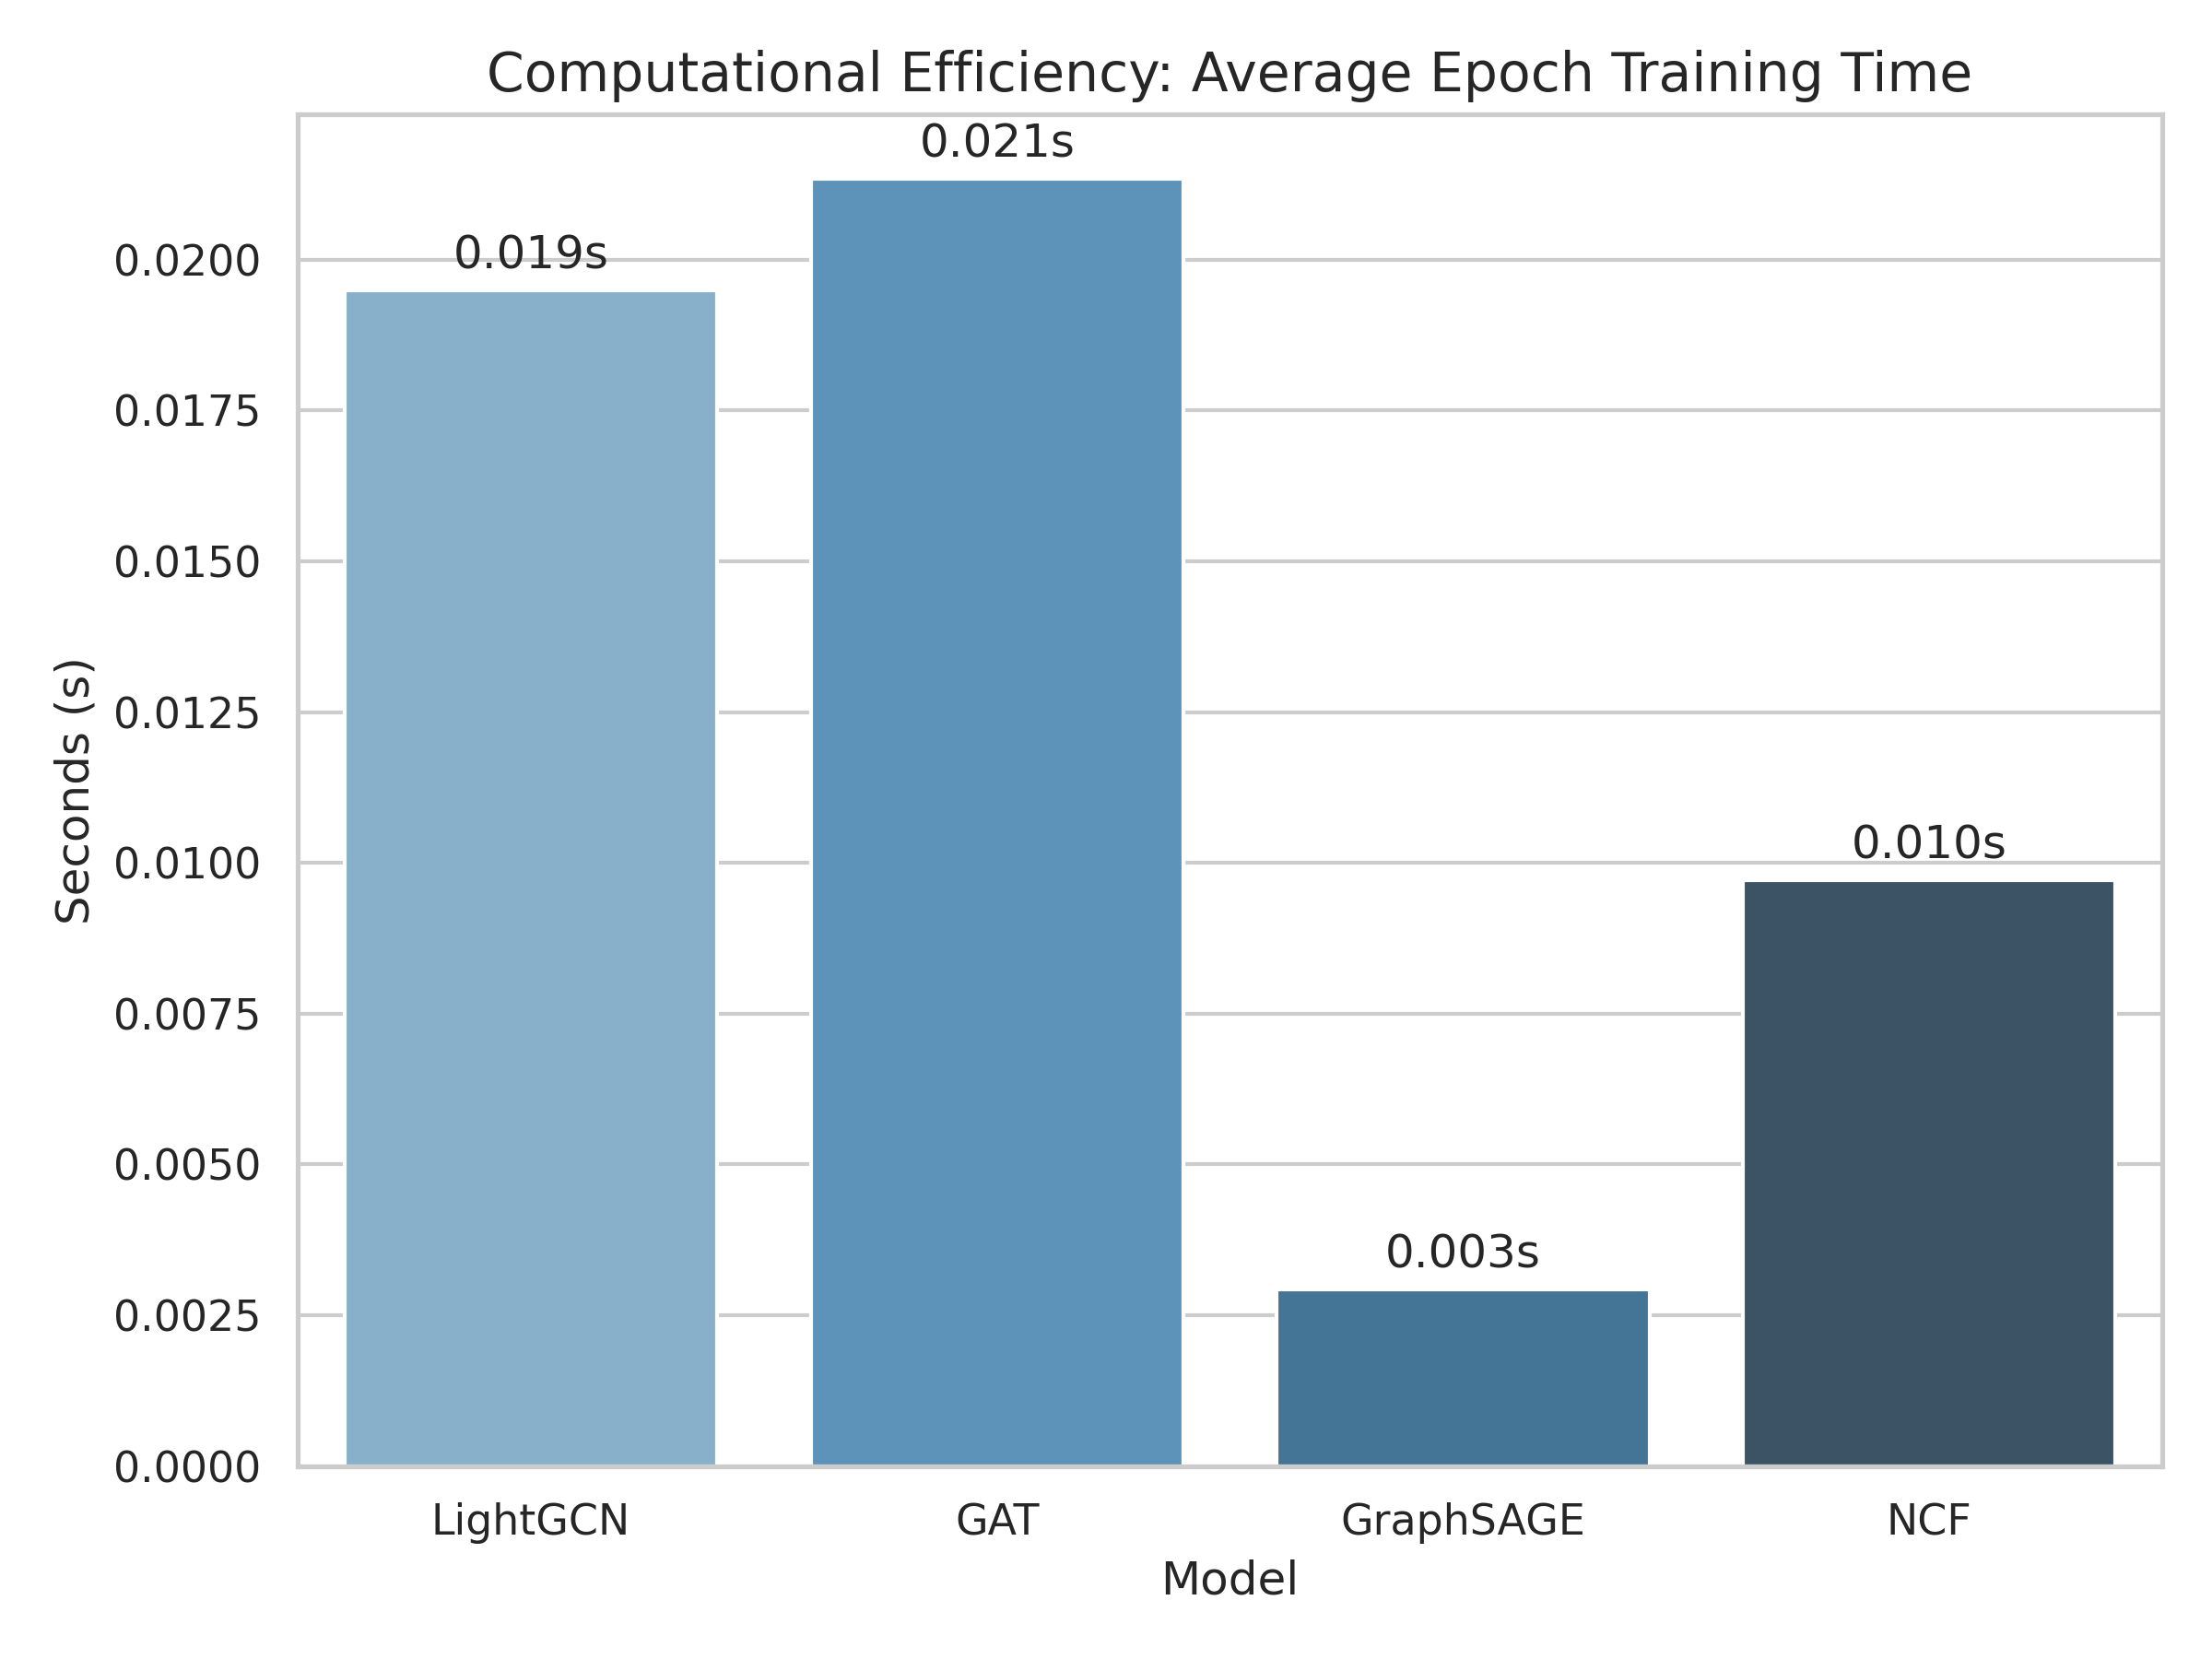
\includegraphics[width=\linewidth]{plots/hardware_epoch_time.png}
        \caption{Average Epoch Training Time}
        \label{fig:time}
    \end{minipage}
\end{figure}

Furthermore, hardware profiling (Figures \ref{fig:vram} and \ref{fig:time}) shows NCF consumes the most peak VRAM ($\approx 4.8$ GB). GraphSAGE proved to be the fastest in terms of per-epoch training time, demonstrating the efficiency of mean-aggregation without attention or heavy factorization components.

\begin{table}[H]
    \centering
    \begin{tabular}{l c c c p{4cm}}
    \toprule
    \textbf{Model} & \textbf{NDCG@20} & \textbf{Recall@20} & \textbf{F1} & \textbf{Notes} \\
    \midrule
    LightGCN & 0.943 & 0.875 & 0.467 & Best ranking performance. \\
    GAT & 0.918 & 0.870 & 0.333 & Implemention complete. \\
    GraphSAGE & 0.925 & 0.869 & 0.333 & Fastest epoch time. \\
    NCF & 0.896 & 0.859 & 0.698 & Best F1, but worst NDCG/Recall. Highest VRAM. \\
    \bottomrule
    \end{tabular}
    \caption{Initial Baseline Results on Test Set}
\end{table}

\section{Planned Improvements and Technical Direction}
For the next phase, my technical direction involves diving deeper into the LightGCN architecture. Since LightGCN currently performs the best, I want to investigate hyperparameter optimization, specifically tuning the number of message-passing layers and the message dropout \cite{he2020lightgcn}. I am also considering adding a margin-based BPR (Bayesian Personalized Ranking) loss explicitly to see if ranking metrics improve further, rather than basic binary cross entropy. If time allows, I might introduce user demographics or movie genres as side features.

\section{Ablation and Error Analysis Plan}
Since LightGCN aggregates embeddings across multiple hops, I plan to ablate the number of layers to understand how high-order connectivity impacts recommendation accuracy versus over-smoothing constraints. I have also developed an \texttt{embedding\_size\_analysis.py} script directly executing an ablation on the embedding sizes (testing ranges from 16 to 128) across models to track capacity ceilings.

\begin{figure}[H]
    \centering
    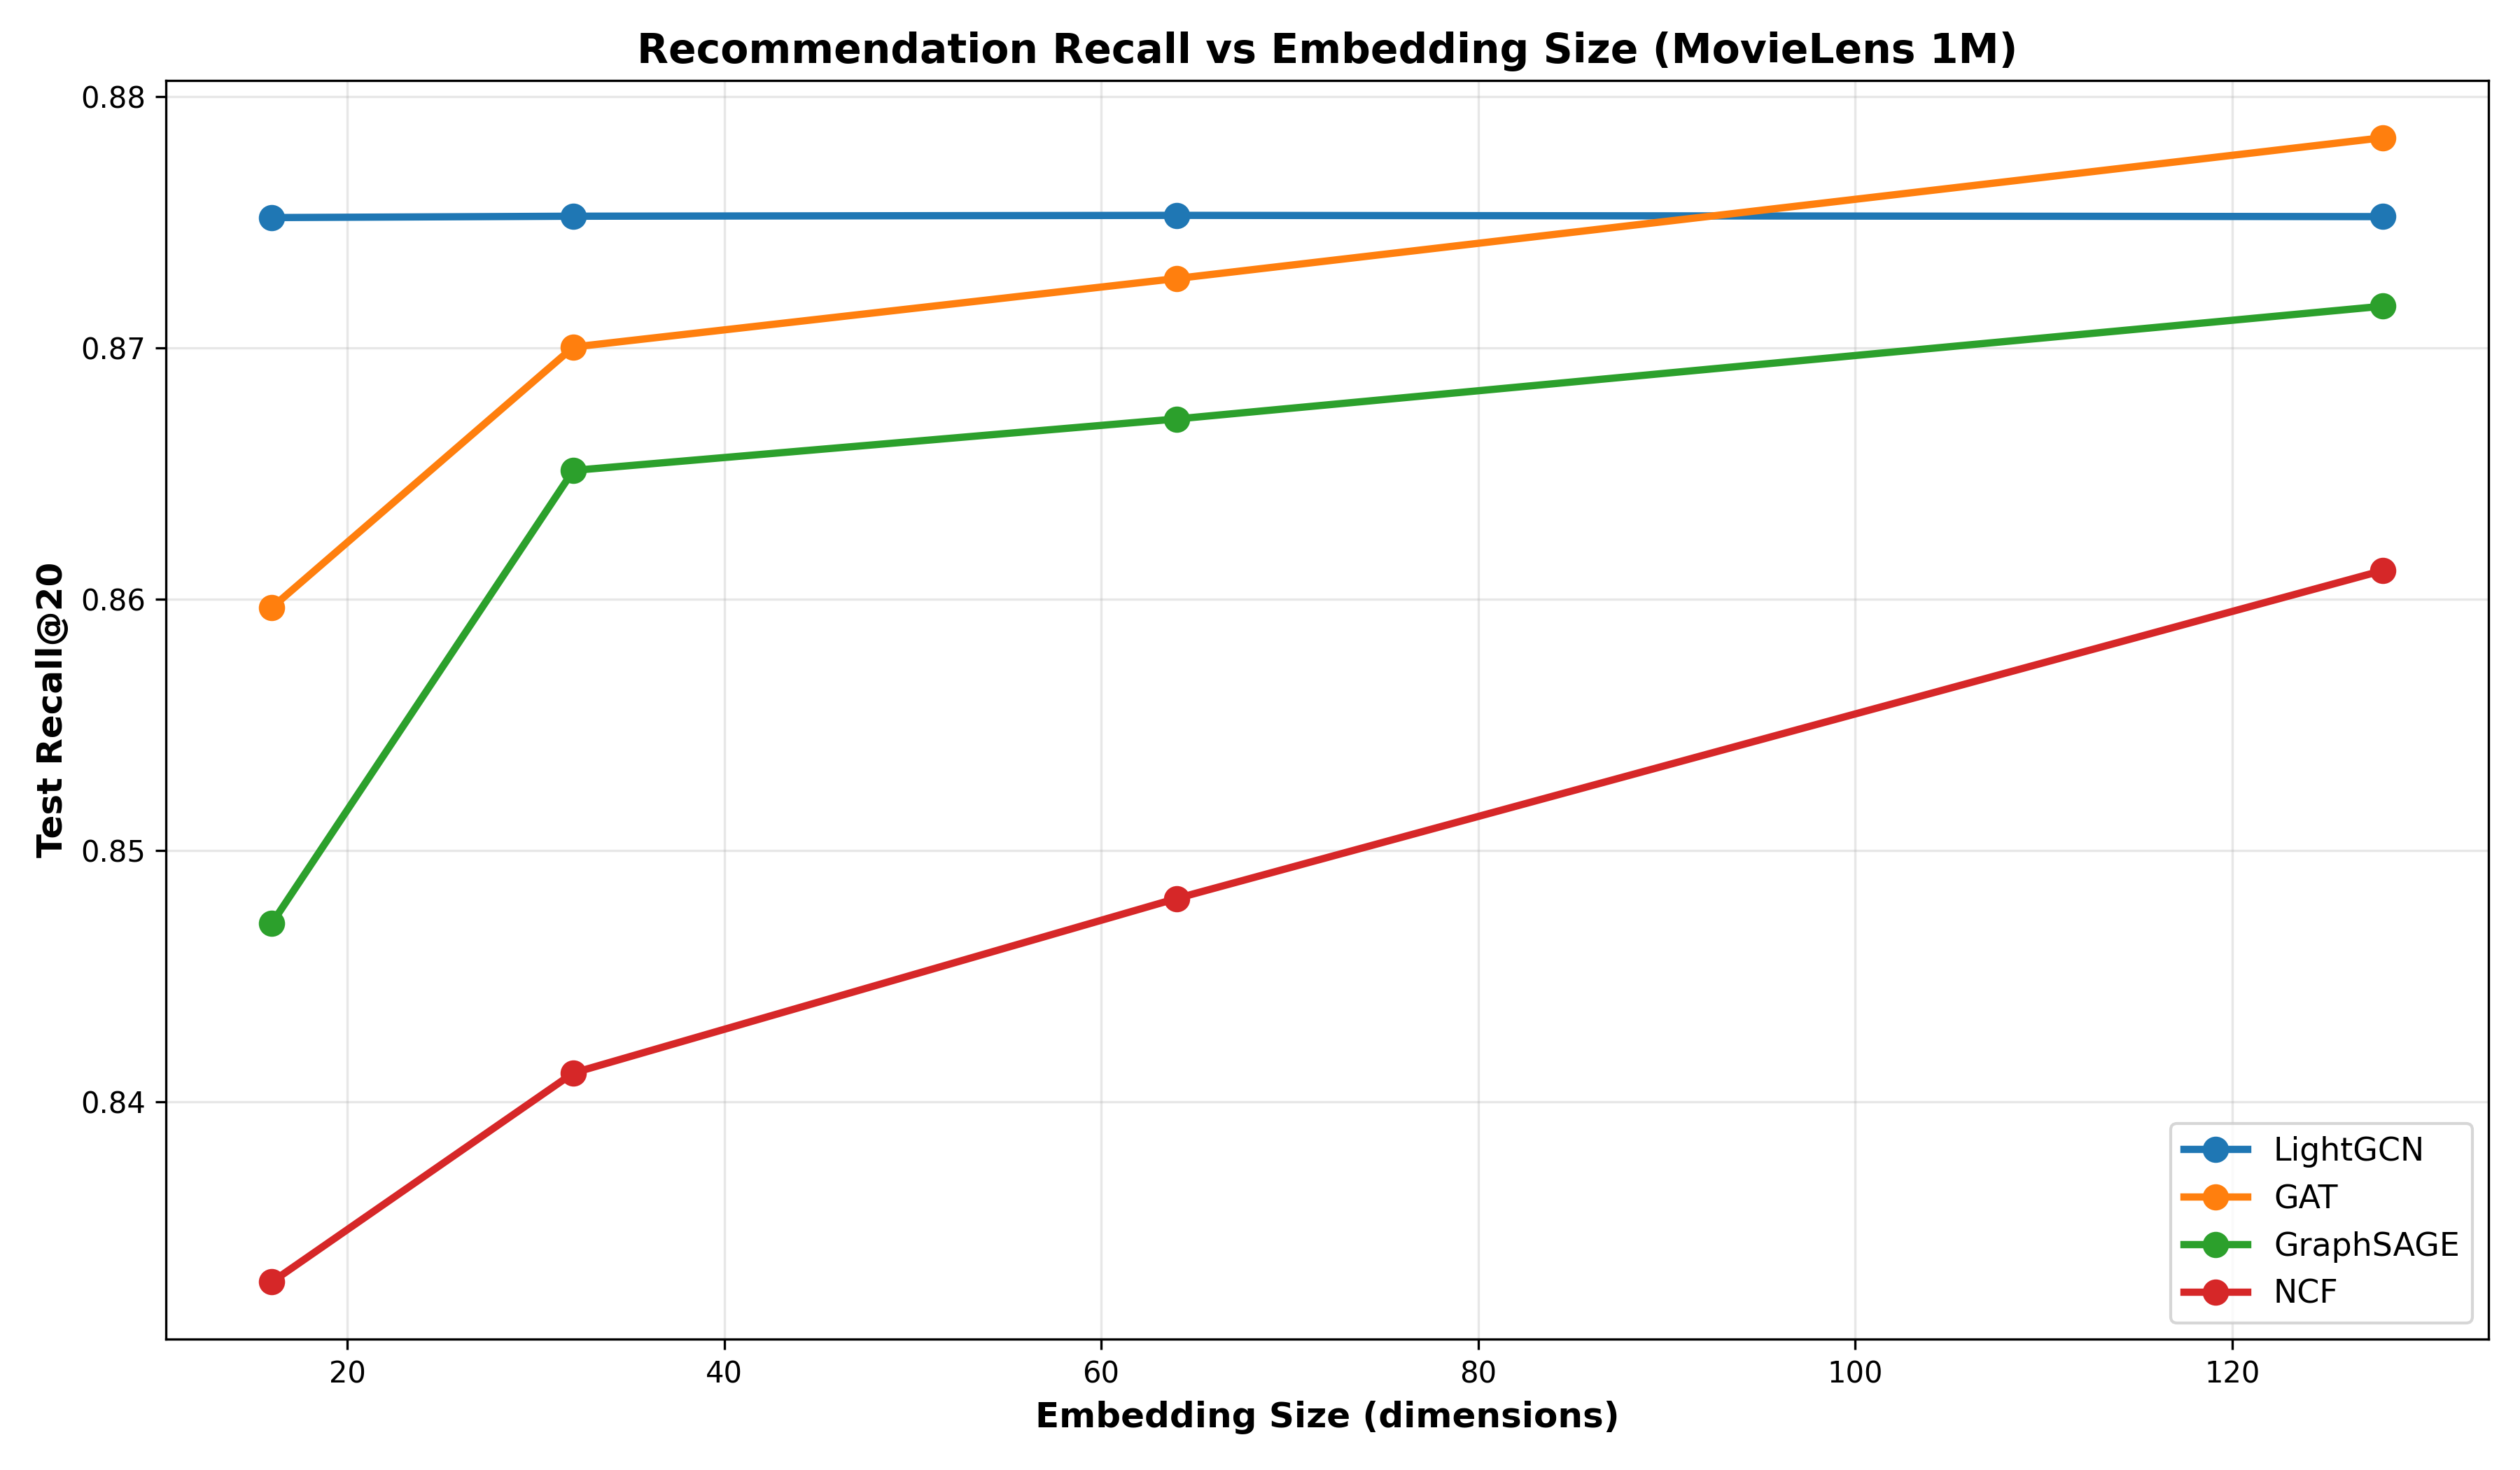
\includegraphics[width=0.78\linewidth]{plots/recall_vs_embedding_size.png}
    \caption{Recall@20 as a Function of Embedding Size}
    \label{fig:recall-embedding}
\end{figure}

Figure \ref{fig:recall-embedding} complements the aggregate heatmap by showing the same ablation as a continuous trend across embedding sizes. This view makes it easier to justify the model-capacity choice in the rest of the report: recall improves consistently as the embedding dimension increases from 16 to 64, indicating that larger latent spaces help the models encode finer-grained user--item preferences. However, the slope becomes less steep beyond 64 dimensions, which suggests diminishing returns relative to the added memory and training cost. This is especially important for the later hardware discussion, because it motivates selecting 64-dimensional embeddings as a practical balance between recommendation quality and computational efficiency.

\begin{figure}[H]
    \centering
    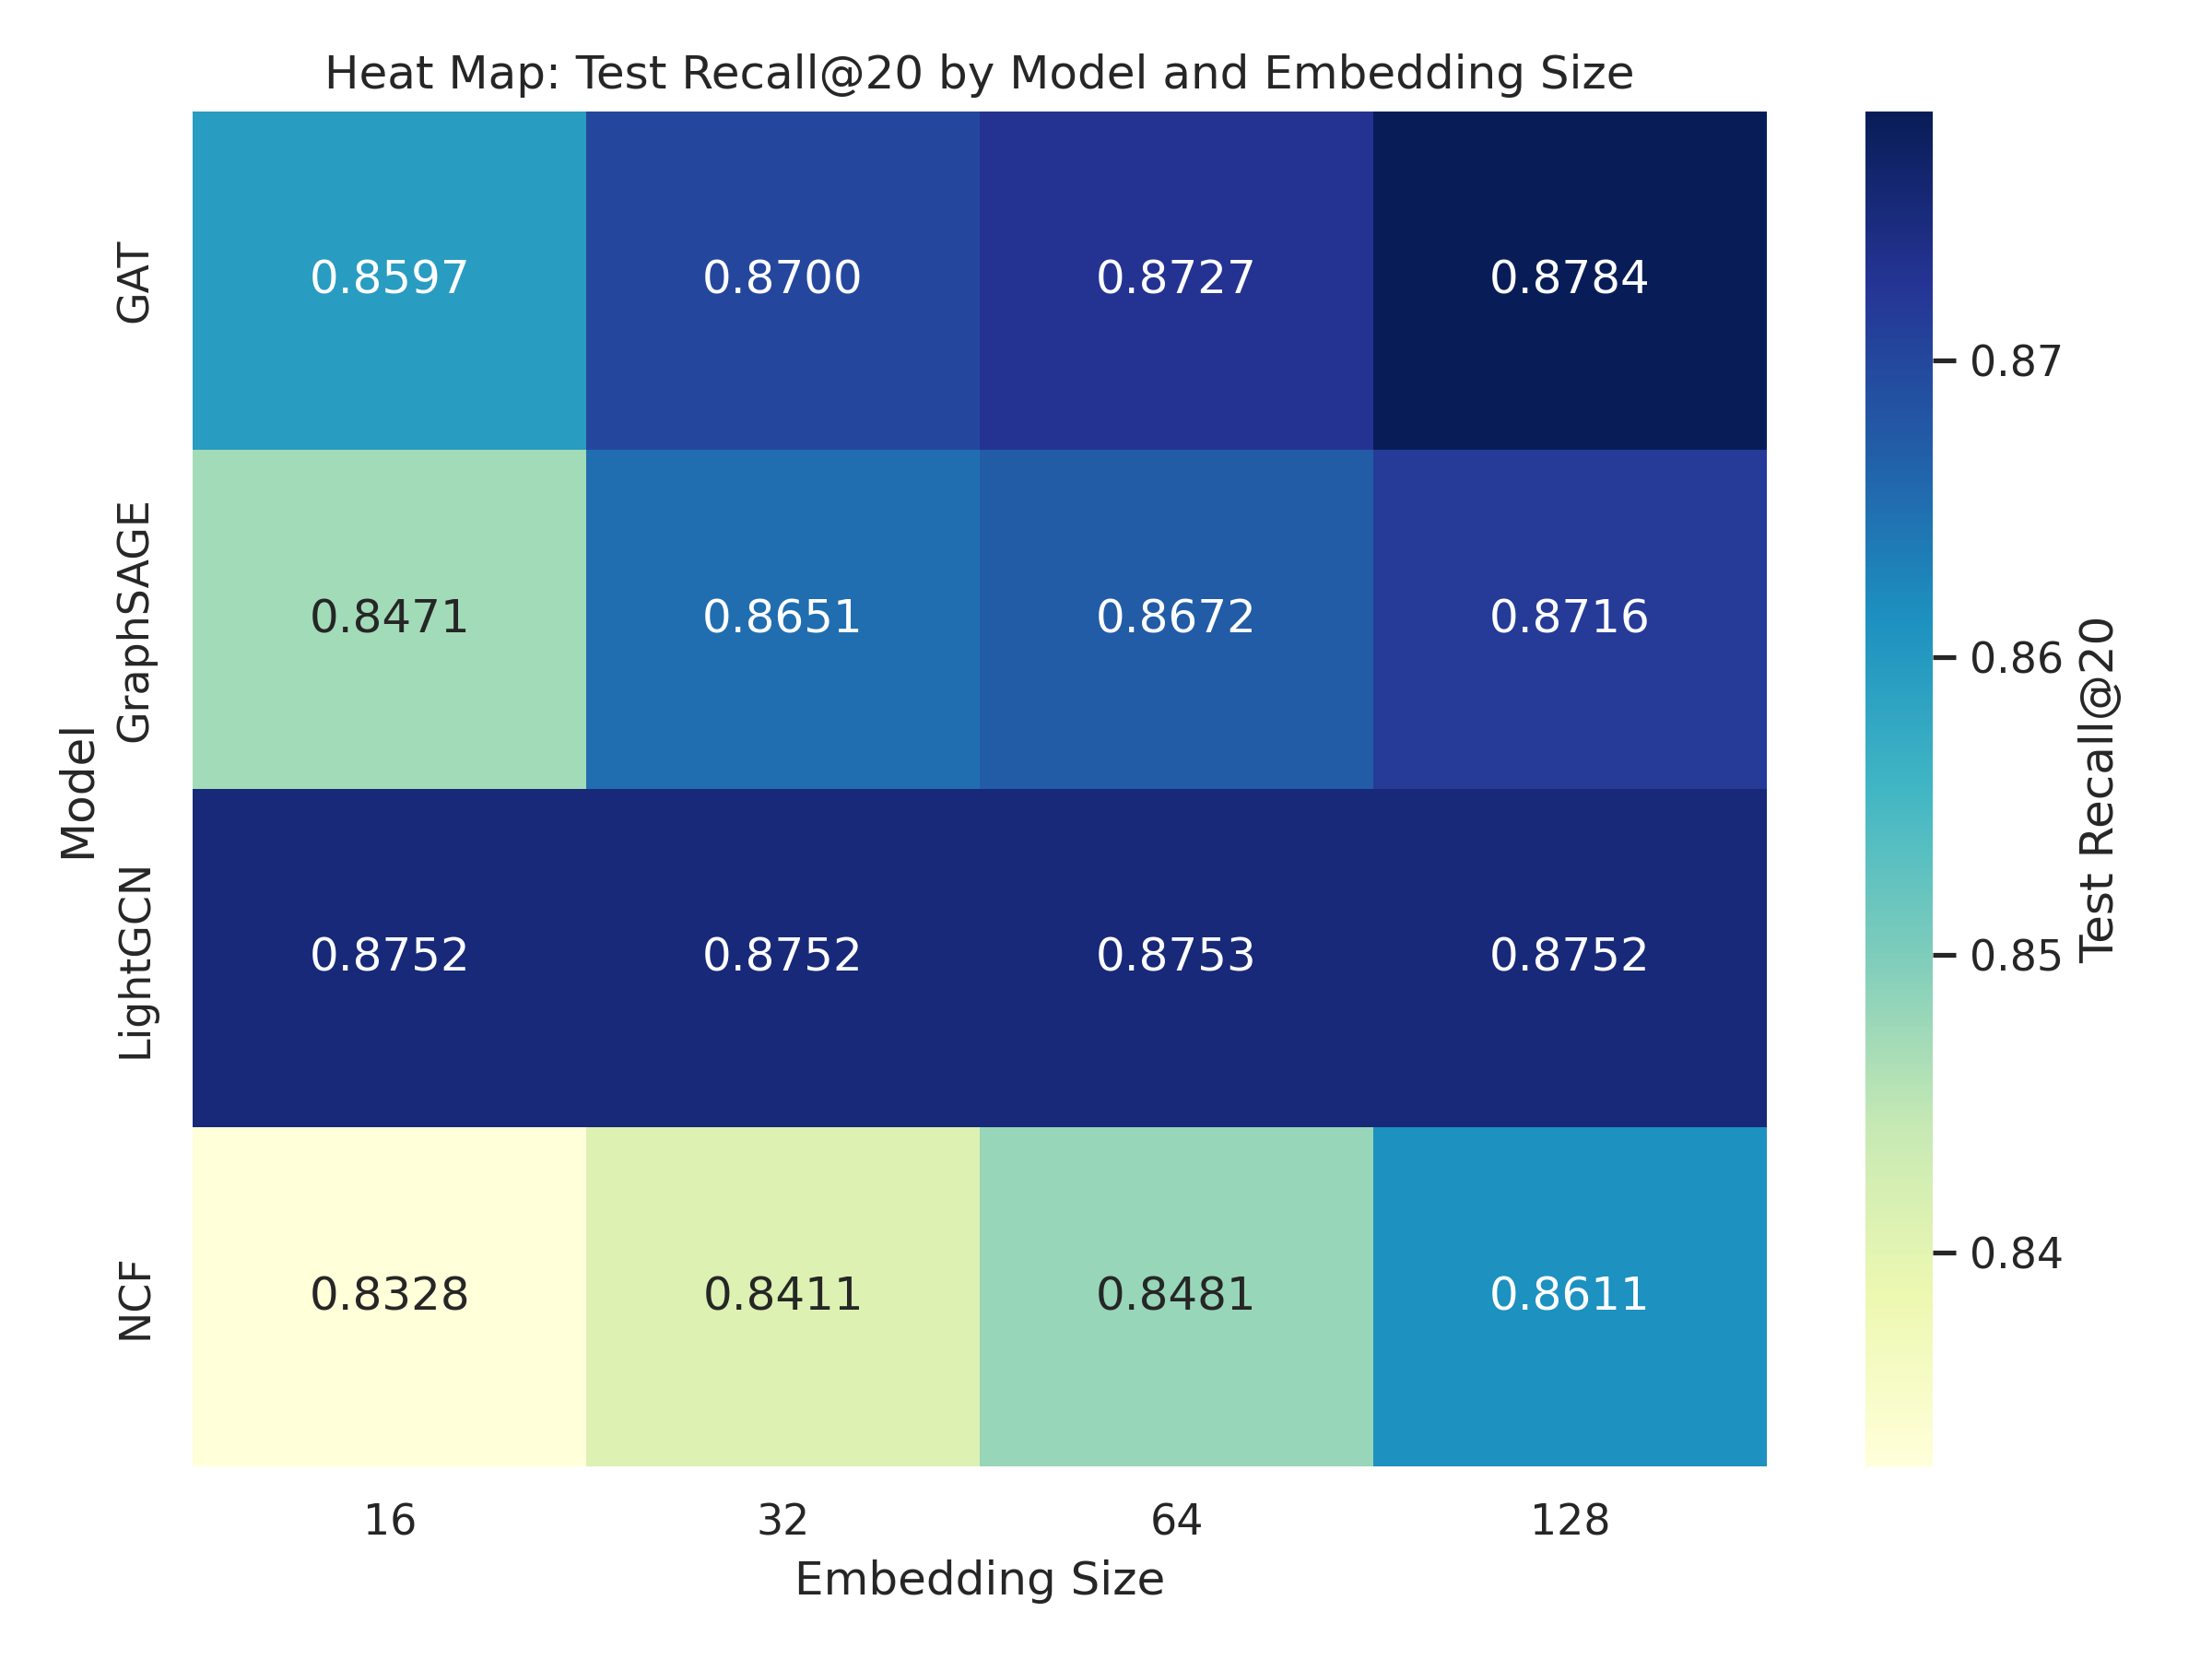
\includegraphics[width=0.75\linewidth]{plots/embedding_size_heatmap.png}
    \caption{Embedding Size Ablation on Test Recall@20}
    \label{fig:heatmap}
\end{figure}

As depicted in Figures \ref{fig:recall-embedding} and \ref{fig:heatmap}, increasing the embedding dimensionality systematically improves Recall@20 across all models, though marginal returns diminish past dimensions of 64. The line plot highlights the growth trend directly, while the heatmap makes the cross-model comparison more compact. Together, they show that LightGCN consistently leverages larger embeddings most effectively.

For error analysis, I have already generated an \texttt{inspection\_report.txt} that logs specific user recommendation evaluations (e.g., retrieving Top-K recommended movie nodes against held-out positive ground truths). By tracing outputs for arbitrary users, I can qualitatively spot-check logical failures. Further, I will investigate the long-tail distribution of the dataset, dividing users into cold-start and highly active sectors to dissect Recall metric divergences per group.

One representative inspection example is user node \texttt{1422}, whose embedding preview begins with small but non-zero latent coordinates (e.g., \texttt{[-0.0097, 0.0116, 0.0116, -0.0139, \dots]}), indicating that the model is encoding preference information in a distributed way rather than through a single dominant feature. For this user, the held-out positives span multiple genres, including \emph{Coma} (Thriller), \emph{Funny Farm} (Comedy), \emph{The Hustler} (Drama), and \emph{Sanjuro} (Action/Adventure). The top-ranked recommendations include titles such as \emph{One Flew Over the Cuckoo's Nest}, \emph{The Grifters}, and \emph{Dances with Wolves}, which suggests that the model recovers a coherent mixture of drama-oriented and classic-cinema preferences. Although the exact held-out list and top-10 recommendation list do not perfectly overlap, this user-level case is still consistent with the aggregate metrics: the quick validation recall reached \texttt{0.8738}, and the quick test run produced approximately \texttt{Recall@20 = 0.8744}, \texttt{NDCG@20 = 0.9410}, and \texttt{F1 = 0.4527}. This strengthens the interpretation that the model is ranking relevant items near the top even when strict classification-style agreement remains lower than ranking-based performance.

\section{Visualization and Interpretation}
I integrated automatic python visualizers that effectively translate numerical results into direct performance interpretations. Instead of standalone numbers, my generated bar charts (like \texttt{ranking\_accuracy.png}) immediately contrast complex ranking metrics. For the embedding ablation, the \texttt{recall\_vs\_embedding\_size.png} figure emphasizes the overall Recall@20 trend as model capacity grows, while \texttt{embedding\_size\_heatmap.png} provides a compact cross-model summary of the same experiment. In addition to these aggregate views, the qualitative inspection logs help interpret what the learned embeddings mean for individual users by connecting numerical metrics to concrete recommendation lists. Also, the pipeline employs \texttt{hardware\_vram.png} profiles to objectively evaluate memory and runtime complexities. These are tied together visually using Mermaid syntax architecture diagrams depicting my underlying model pipeline.

\section{GitHub and Reproducibility Status}
My project places a strong emphasis on full reproducibility and transparent environment management. I am actively tracking all my experimental configurations, training scripts, and plotting dependencies in a dedicated GitHub repository through continuous commits. The project repository is available at \href{https://github.com/heneka/project-463}{github.com/heneka/project-463}. For my local development setup, I am running the computational pipeline within the Windows Subsystem for Linux (WSL) and utilizing an RTX 5070 laptop GPU, which significantly accelerates the training of the multi-hop graph models. 

To ensure that anyone can perfectly replicate my environment and results, I am using \texttt{uv} paired with Python's native \texttt{venv} module for fast, isolated virtual environment management. I have also generated a clean \texttt{requirements.txt} file that specifies the exact tailored dependencies needed to run the project. Furthermore, all core hyperparameter settings—such as evaluation bounds, epochs, and learning rates—are centrally and uniformly managed within a \texttt{config.yaml} file. This structure allows the primary execution scripts (\texttt{main.py} and \texttt{visualize.py}) and the modular \texttt{src/} directory to be run instantly by anyone syncing the repository.


\section{Current Challenges and Next Steps}
My primary challenge right now surrounds a bizarre evaluation discrepancy where NCF captures lower NDCG scores but much higher unweighted F1 scores compared to my varied graph modules. This is likely tied to the logit thresholding logic applied against negative samples, and tracing it requires granular investigation; this kind of mismatch between link-prediction-style classification behavior and Top-K recommendation quality is also discussed in prior work \cite{yuan2024dotproduct}. 

The user-level inspection example reinforces this issue: even when the recommendation list is semantically plausible and the ranking metrics are strong, the overlap-based classification signal can still look comparatively weaker. This confirms that part of the discrepancy is methodological rather than purely qualitative, so the next debugging step is to examine threshold calibration and the construction of negative samples more carefully.

My specific technical goals bridging towards final submission involve formally integrating Bayesian Personalized Ranking (BPR) Loss for structural ranking improvement. I will also expand upon my \texttt{embedding\_size\_analysis.py} to finalize the comprehensive embedding and graph-layer ablations. Finally, I will formalize the long-tail dataset evaluations formulated within my raw \texttt{inspection\_report.txt} into empirical distribution metrics.

\begin{thebibliography}{9}

\bibitem{he2020lightgcn}
He, X., Deng, K., Wang, X., Li, Y., Zhang, Y., \& Wang, M. (2020).
\textit{LightGCN: Simplifying and Powering Graph Convolution Network for Recommendation}. 
In Proceedings of the 43rd International ACM SIGIR Conference on Research and Development in Information Retrieval (pp. 639–648).

\bibitem{he2017neural}
He, X., Liao, L., Zhang, H., Nie, L., Hu, X., \& Chua, T. S. (2017).
\textit{Neural Collaborative Filtering}. 
In Proceedings of the 26th International Conference on World Wide Web (pp. 173–182).

\bibitem{hamilton2017inductive}
Hamilton, W., Ying, Z., \& Leskovec, J. (2017).
\textit{Inductive Representation Learning on Large Graphs}. 
Advances in Neural Information Processing Systems (NeurIPS), 30.

\bibitem{velickovic2018graph}
Veličković, P., Cucurull, G., Casanova, A., Romero, A., Lio, P., \& Bengio, Y. (2018).
\textit{Graph Attention Networks}. 
International Conference on Learning Representations (ICLR).

\bibitem{hu2023graphcross}
Li, H., Wang, S. et al. 
\textit{Graph Cross-Correlated Network for Recommendation}. 
Available as relevant conference proceedings or pre-prints in literature relating GNN representation tracking.

\bibitem{shafiq2023review}
Shafiq, O. et al. 
\textit{A Review on Multi-Types Analysis for Graph Neural Networks-Based Recommendation Systems}. 
Survey of GNN adaptation methodologies for heterogeneous structures.

\bibitem{yuan2024dotproduct}
Yuan, B., \& et al. 
\textit{Dot Product is All You Need: Bridging the Gap Between Item Recommendation and Link Prediction}. 
Discusses the evaluation dichotomy between link-prediction classification bounds and recommendation ranking lists.

\end{thebibliography}

\end{document}
